%\subsection{Workflow}
\label{sec:workflow}


\begin{figure}
\centering
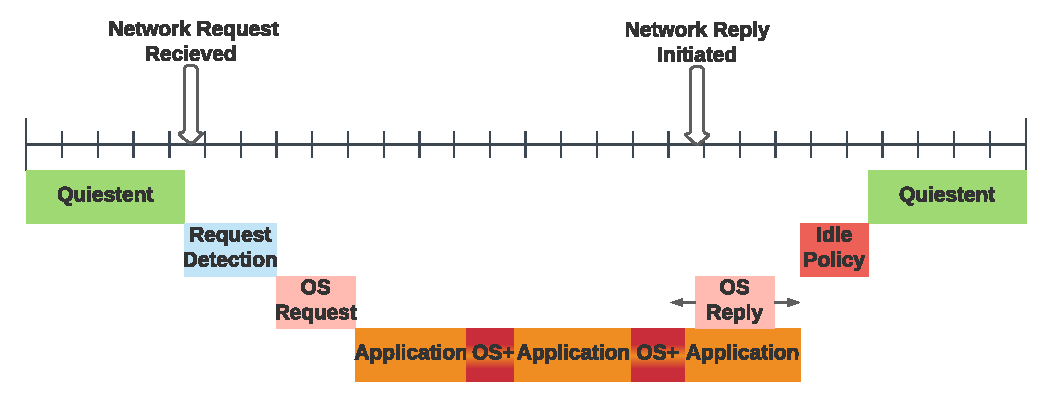
\includegraphics[width=0.5\textwidth]{figures/timeline_chart}
\caption[]{W timeline for a single application request}
\label{fig:timeline}
\end{figure}

From an OS perspective we break down network driven processing into stages that allows us to organize and reflect the OS and application interaction with the workload request timeline.  This break down is illustrated in figure~\ref{fig:timeline}.   

\subsection{Quiescent}
Given the packet and transactional nature of network driven services a quiescent period, in which no requests are present at the server, precedes activity on the server. 

\subsubsection{Open Loop:}
In an open loop scenario like a Memcached workload, the external request rate induces an inter-arrival gap that will drive the quiescent period -- longer at lighter loads (lower queries per second (QPS)) and shorter at heavier loads (higher QPS). Largely the arrival rate can be considered independent of the time required to service a request.  System performance is typically evaluated in terms of the 99\% tail latency it achieves.  Moreover, providers often set a Quality of Service (QoS) target, such as  a 99\% tail latency of 500${\mu}$s, categorizing system performance into acceptable and unacceptable.  As Mootaz et al.\cite{mootaz} observed, in latency focused workloads, the "latency-slack" between the mean time to servicing a request and the QoS target creates an opportunity for energy-performance tradeoffs.  In particular, it maybe possible to reduce mean performance by not executing requests as fast as possible and or not processing request immediately upon their arrival to reduce energy consumption while not violating the QoS target.  

\subsubsection{Closed Loop:}
In a closed loop setting, like snapshotting a database to a remote server or video streaming, the arrival rate of the next request, that forms the overall task, depends on how long it takes to service the current request.  However, the quiescent period is bounded by the network round trip time, that depends on  the size of a request and reply packets, and the remote processing time.   System performance is largely evaluated on how fast a server can complete the entire task given a network link speed and a remote system.  Given workload specific characteristics such as the processing required and round-trip costs it is possible, as we will see, to find configurations in which the OS interacts with slowing down to improve both time and energy.   Often research tends to categorize close loop settings as either not representative of cloud computing or imply that energy-performance tradeoffs are not interesting due to the hight utilization closed-loop processing can imply.  

Given our goal of studying and explaining the implications of the OS on network driven processing our analysis framework, and evaluation, includes closed loop settings.  In particular, we use a simple ping-pong application to stress OS behavior while varying packet-sizes to reveal how OS path length and path efficiency interacts with slowing down processing, relative to the round trip time observed at the server.  Additionally we use a second closed loop that stresses single core application processing with negligible packet sizes to evaluate if OS structure can impact the application efficiency.  

 
\subsection{OS Request Detection}

Fundamental to any operating system is how it detects and schedule processing in response to IO device activity.  At the two extremes are interrupt and poll driven detection.  

\subsubsection{Interrupt driven IO}
Using interrupts has three important implications: 1) Interrupts can be used to transition a processor from a halted state which the OS entered to sleep the processor (at some selected HW sleep state (C-state)) in response to external activity, 2)  Interrupts allow an OS to arbitrate processing across competitive devices and processing in a multi-programmed/multi-device setting, 3) interrupt processing has an inherent performance costs associated with it -- in terms of latency in starting handling of a request, either because of the costs associated with preempting currently scheduled work\cite{intelpaper} or exit penalties associated with the C-state that the processors was halted in\cite{}.  Interrupt processing can also have a negative impact on the instruction efficiency, measured in Instructions Per Cycle (IPC), due to induced micro-architecture hazards such as the inability to prefetch or speculatively execute across an interrupt.

\subsubsection{Poll driven IO}

Most modern high-speed devices expose a memory, if not cache, friendly interface, that permits the processors to read a per-core memory address to determine if the device, such as the Network Interface Card (NIC) has received data that requires processing by the core.  This facility allows software to directly poll the device and initiate software handling without an interrupt.  This approach reduces latency and other performance penalties associated with interrupt driven IO.  However, the period in which the device is checked requires CPU activity and thus limits the ability to halt the cores when there is no work to be done.  In the extreme, a customized OS, supporting a single application can run a poll loop on every core to constantly check for work, conduct the work and then go back to polling for new work and thus never halting the processors due to idleness.   While used in a slightly different context to Kim et al.\cite{hank}, we will refer to this regime as 'no-idle', as it results in a similar energy management strategy albeit in the context of network driven processing.  In general such an aggressive poll approach is assumed to maximize performance by avoiding interrupt overheads and minimizing latency. 

\subsubsection{Hybrid driven IO}
% https://wiki.linuxfoundation.org/networking/napi
A general purpose operating system typically exploits some form of hybrid alternating between using interrupts and polling when servicing high speed NICs. A common strategy is to use interrupts when load is low and switch to polling when load is high and back to interrupts when load reduces.  A general purpose OS, even under sustained high load, bounds the poll phase to avoid the starvation of other devices and computation.  In Linux the framework that implements this hybrid scheme for is called New API (NAPI)\cite{NAPI}.  The first arrival of a packet generates an interrupt which switches the servicing of the device to polling for some budget of packets and time after which the device will no longer be polled and interrupts re-enabled to detect activity on the NIC.  The NAPI framework, in addition to NIC processing budgets,  supports prioritization across devices. 
% In Linux the NAPI polls are processed via softirqs.  Checks for and processing of softirqs happens when ever the system returns to userspace or a hardware interrupt exits.

A library OS that is specialized to support the execution of a single application in the context of a fixed dedicated NICS can explore more extreme strategies like aggressive polling, described above, given that it need not arbitrate the device or cores.

\subsubsection{Interrupt Delaying}
\tikzstyle{startstop} = [rectangle, rounded corners, minimum width=3cm, minimum height=1cm,text centered, draw=black, fill=red!30]
\tikzstyle{io} = [trapezium, trapezium left angle=70, trapezium right angle=110, minimum width=3cm, minimum height=1cm, text centered, draw=black, fill=blue!30]
\tikzstyle{process} = [rectangle, minimum width=3cm, minimum height=1cm, text width=2cm, text centered, draw=black, fill=orange!30]
\tikzstyle{decision} = [diamond, minimum width=3cm, minimum height=1cm, text width=1cm, text centered, draw=black, fill=green!30]
\tikzstyle{arrow} = [thick,->,>=stealth]

%\begin{figure}
\centering
%\resizebox{5cm}{3cm}{%
\begin{tikzpicture}[node distance=2cm]

\node (start) [startstop] {ITR=\textit{n} $\mu$s};
\node (dec1) [decision, below of=start] {ITR==\textit{0}?};
\node (pro1) [process, right of=dec1, xshift=1.5cm] {ITR-=\textit{2} $\mu$s};
\node (dec2) [decision, below of=dec1, yshift=-0.5cm] {RX/TX Event?};
\node (pro2) [startstop, left of=dec2, yshift=1.5cm, xshift=-0.8cm] {Assert Interrupt};

\draw [arrow] (start) -- node[anchor=west] {check} (dec1);
\draw [arrow] (dec1) -- node[anchor=north] {no} (pro1);
\draw [arrow] (pro1) |- node[anchor=west] {update} (start);
\draw [arrow] (dec1) -- node[anchor=west] {yes} (dec2);
\draw [arrow] (dec2) edge[loop right]node{no} (dec2);
\draw [arrow] (dec2) -- node[anchor=east] {yes} (pro2);
%\draw [arrow] (pro2) -| node {} (start);
\draw [arrow] (pro2) |- node[anchor=east] {reset} (start);
\end{tikzpicture}
%}
%\vspace*{-5mm}
%\caption{ITR-Delay algorithm flowchart.}
%\label{fig:itr_delay_flowchart}
%\vspace{-.25in}
%\end{figure}
A common feature of modern high speed NICs is the ability to delay the delivery of interrupt when an event such as packet arrival or transmission completion.  By manipulating this setting software can limit the minimum time between interrupts or in other words the maximum rate at which the NIC events can interrupt the CPUs.    The NIC we use in this study exposes this mechanism via an Interrupt Throttling (ITR) setting.  We flowchart the algorithm from the NIC's datasheet~\cite{82599} in  Figure~\ref{fig:itr_delay_flowchart}. Software uses the ITR register to configure a delay in 2$\mu$s increments.  If the spacing of events, such as packet reception, is less than  $2{\mu}s \times ITR$ the NIC will delay assertion.  If on the other hand events are sufficiently separated an interrupt will be asserted immediately.   

By default the Linux device driver attempts to automatically set ITR to reduce interrupt overheads.  We disable this feature and manually control its value to explore the impact of delaying the detection of NIC events.  Combining interrupt driven IO and delaying interrupt assertion via ITR setting we can explore the impact of delaying packet detection and thus delaying processing of requests.  Depending of the state of the processor the NIC can buffer packets in its own memory or on the main memory of the host\footnote{According to the data sheet if the processor is in sleep state packets can only be buffered on the card's limited memory and once exhausted packets will be dropped}.  Delaying interrupt detection introduces an OS control that can interact with energy and performance.  The prior work of Mootaz et al\cite{mootaz} and the more recently work of Chou et al{chou} suggests that delaying packet processing can interact with DVFS and C-State control in latency sensitive workloads to yield useful energy performance tradeoffs. To this end we sweep ITR values for all our workloads OS configurations, and DVFS values.



%\subsection{Application Perspective}
%Figure~\ref{fig:timeline} shows the application is waiting to be woken up to process new packets (a). Next, an interrupt (b) is fired and the OS network stack begins processing the received packet (c). The application level work begins, alongside there are also interspersed OS work which may or may not be in direct support of application(d). The tail end of the application work (e) typically entails a response packet being sent, the period of time with which the response packet is physically sent can proceed in parallel with the rest of the application level work. The end of every request handling (f) also revolves a set of OS policies to decide the next state of the software and hardware. Work is time spent executing instructions required to service a request, it is a function of the software, hardware, and workload itself. Whereas, idle time is a function of arrival rate of packets.
%
%\subsection{Hardware Perspective}
%Slowing down of the processor causes an increase in the time spent in portions of application and OS work while reducing energy use. Slowing down of interrupt delays contributes to the increase of time spent in the idle states, the longer a processor idles the more energy it can save.
%
%\subsection{OS Perspective}
%OSes overall behaviour is a function of how it behaves during both the working and idle portions of time, there also exists a clear inter-relationship between the two. 
%
%The amount of energy used during this idle period is dependent upon the OS idling policies; in terms of which level of idle state is selected.
%
\subsection{Equations}

%\subsection{ITR-Delay algorithm}
